\documentclass[a4paper, 12pt]{article}
\usepackage{amsmath}
\usepackage{amsthm}
\usepackage{amsfonts}

%%% Работа с картинками
\usepackage{graphicx}  % Для вставки рисунков
\graphicspath{{images/}{images2/}}  % папки с картинками
\setlength\fboxsep{3pt} % Отступ рамки \fbox{} от рисунка
\setlength\fboxrule{1pt} % Толщина линий рамки \fbox{}
\usepackage{wrapfig} % Обтекание рисунков текстом

\newtheorem{lemma}{Lemma}
\newtheorem{theorem}{Theorem}
\newtheorem{cor}{Corollary}
\title{Outer billiard outside the regular 7-gon}
\date{2021\\ August}
\author{authors}
\begin{document}
\maketitle
\textbf{Abstract.} Here is some abstract
\section{Introduction}
Let $P$ be a regular 7-gon in $\mathbb{R}^2$ with vertices $\{p_1,...,p_7\}$, let $X=\mathbb{R}^2\setminus P$. Let $f:X\setminus B_0 \rightarrow X$ be a reflection in the rightmost vertex of $P$ where $B_0$ is a ray continuation to the right for each side of the polygon (we denote them $B_{01}$,...,$B_{07}$ where the second index is an index of a base vertex of the ray from the polygon), on $B_0$ the map $f$ is undefined. $B_0$ divides the domain $X$ into domains $D_1,...,D_7$ where subscript is an index of the rightmost vertex.

We say that on $X$ a right outer billiard (outside $P$) is defined when such $f:X\setminus B_0 \rightarrow X$ is defined.

The set $O(x)=\{x,f(x),f^2(x),f^3(x),...\}$ is the orbit of a point $x\in X \setminus P$(If we reach a point in $B_0$, we stop iteration).
\[\text{Let } B_1=B_0 \cup f^{-1}(B_0),\]
\[B_n=B_0\cup f^{-1}(B_0)\cup...\cup f^{-n}(B_0)=B_{n-1}\cup f^{-n}(B_0),\ n \geq 0,\]
\[B_{\infty}=B_0\cup f^{-1}(B_0)\cup...\cup f^{-n}(B_0)\cup...\]

Let us consider a letter sequence (a word) $l_0l_1...l_n...$ from an alphabet $A$, that is for all $ k\ l_k\in A$. Let $FW(A)$ be a set of all finite words over the alphabet $A$ (ex. $l_0l_1...l_n\in FW(A)$), $LFW(A)$ be a set of all left finite words, but they can be not right finite (ex. $l_0l_1...l_n...\in LFW(A)$).

We define a concatenation operator $\ast :FW(A)\times LFW(A)\rightarrow LFW(A)$,\newline
$a\ast c := ac$, $a\in FW(A)$, $c \in LFW(A)$.\newpage
We define a length function $length:LFW(A)\rightarrow \mathbb{N}_0\cup\{\infty\}$; $length(l_0...l_n):=n+1$; $length(l_0...l_n...):=\infty$; $length(ab)=length(a)+length(b)$.

We say that a letter sequence $l_0l_1...l_n...$ where for all $k\ l_k\in \{1,2,...,7,b\}=:A$ is an itinerary of a point x $\in$ X ($it(x):=l_0l_1...l_n...$) when $l_k\neq b \Rightarrow\newline\Rightarrow f^k(x)\in D_{l_k}$, and $l_k = b \Rightarrow f^k(x)\in B_0$ $(f^0(x):=x)$, the sequence ends on $b$ or is infinite; for all $k$ $l_k$ is called a $k$-th address.

We say that a point $x\in X\setminus B_0$ is periodic if there is $k>0$ s.t $f^k(x)=x$, $k$ is called a period, $\min\{k_1,k_2,...\}$ of such $k_i$ is called a prime or least period.

We say that a point $x\in X\setminus B_0$ is aperiodic if there is no $k>0$ s.t. $f^k(x)=x$\newline
$f(B_k\setminus B_0)=B_{k-1}$, $k>0$.
\section{Itineraries}
We consider $S_a=\{x\in X\setminus B_0|\ it(x)=a...\}$ for some $a=a_0a_1...a_k$ where $a_k\neq b$ that means that $S_a$ is a set of all points s.t. their itineraries begin with $a$.\newline
\begin{lemma} The map $f^{k+1}$ is defined on $S_a$.
\end{lemma}
\begin{proof} For all $x \in S_a$ there exists $r(x)$ s.t. $it(x)=a_0a_1...a_kr(x)$ by definition of $S_a$. By definition of an itinerary, $it(f^{k+1}(x))=r(x)$. Hence, $f^{k+1}$ is defined on $S_a$.
\end{proof}
\begin{lemma} The map $f^{k+1}$ is undefined on $\partial S_a$ ($\partial$ denotes the boundary of a set).
\end{lemma}
\begin{proof}  Let $S_a^k=f^k(S_a)$. We have $S_a^k=\{x| x\in D_{a_k}\}$. Hence, $\partial S_a^k\setminus \partial P= B_{0\ (a_k-1)\ mod\ 7}\cup B_{0a_k}$(there can be a case when $\partial S_a^k\cup \partial P\neq \emptyset$). Also $f^k(\partial S_a\setminus \partial P)=\partial S_a^k\setminus \partial P$. The map $f$ is undefined on this set. Hence, $f^{k+1}$ is undefined on $\partial S_a$.
\end{proof}
\begin{cor} The boundary of $S_a$ is a subset of $B_k\cup \partial P$(direct implication of the proof of the lemma 3).
\end{cor}
\begin{cor} The set $S_a$ is an open polygon.
\end{cor}
\begin{lemma} All components of $X\setminus B_k$ are convex.
\end{lemma}
\begin{proof}
For two fixed points $x,y$ we consider a closed interval $[x,y]:t=$\newline
$=(1-\alpha)x+\alpha y$, where $\alpha\in\mathbb{R}$ is continuously changing from 0 to 1.

Let us assume that there exists a component $D$ that is not convex.
That means that we can find two points $x,y\in D$ s.t. the interval $[x,y]$ will have a point $z=(1-\alpha_0)x+\alpha_0 y\not \in D$.

The component $D\subset D_i$ for some $i$, hence, $[x,y]\subset D_i$, $f(x)=2p_i-x$ for $x\in D$.

The map $f$ takes any interval in $D_i$ and returns an interval in $X$.

By the assumption we conclude that $[x,y]\cap B_{n_0}\setminus B_{n_0-1}\neq \emptyset$ for some $0<n_0\leq k$.

Generally there can be more intersections with other $B_{n_1},B_{n_2}...$, for simplicity we will consider only $n_0$ and assume that it is minimal, further we will show that even with such single $n_0$ we get a contradiction. For each $n\leq n_0-1\ f^n([x,y])\cap B_{n_0-n}\setminus B_{n_0-1-n}\neq \emptyset$ and $f^n([x,y])\cap B_{n_0-1-n}=\emptyset$ (because we chose minimal $n_0$). This statement implies that $f^n([x,y])$ is entirely inside one of the domains $D_1,...D_7$, hence,  $f^n([x,y])=[f^n(x),f^n(y)]$ is an interval. In particular, $f^{n_0-1}([x,y])=[f^{n_0-1}(x),f^{n_0-1}(y)]$. The interval $[f^{n_0-1}(x),f^{n_0-1}(y)]$ is placed inside one of the domains $D_1,...D_7$ and has an intersection with $B_1$. And finally $f^{n_0}([x,y])=[f^{n_0}(x),f^{n_0}(y)]$ is an interval.

That means $f^{n_0}(x)\in D_i,\ f^{n_0}(y)\in D_j,\ i\neq j$.

And we reach a contradiction because the $n_0$th-addresses are different, but we know that any two points of the same component of $X\setminus B_k$ will stay in the same component until $f^k$, hence, all the addresses until the $k$th-address must be the same.\newline
\end{proof}
\begin{cor} The set $S_a$ is convex.
\end{cor}
\begin{theorem} We suppose that k is even, that $S_a$ has a point $x_0$ that has $it(x_0)=aac$ for some c. Then $S_a$ has a periodic point with period k+1.
\end{theorem}
\begin{proof} So we have the point $x_0$ with the itinerary $aac$.\newline
Since $x_0\in S_a$ and $f^{k+1}(x_0)\in S_a$, $S_a$ and  $f^{k+1}(S_a)$ intersect.\newline
The map $f^{k+1}$ on $S_a$ is a reflection:\newline
\[f^{k+1}(x)=2\sum\limits_{i = 0}^{k}(-1)^{k}(-1)^{i}p_{a_i}+(-1)^{k+1}x=2\sum\limits_{i = 0}^{k}(-1)^{i}p_{a_i}-x,\]
\[p^{\ast}:=\sum\limits_{i = 0}^{k}(-1)^{i}p_{a_i}=\text{const for } x\in S_a.\]
The intersection yields that there is a point $x\in S_a$ s.t.
\[f^{k+1}(x)=2p^{\ast}-x=y\in S_a.\]
It implies that $p^{\ast}=\frac{x+y}{2}$. From the corollary about convexity of $S_a$ it implies that $p^{\ast}\in S_a$. In that case, $f^{k+1}(p^{\ast})=2p^{\ast}-p^{\ast}=p^{\ast}$. That means that $p^{\ast}$ has period $k+1$.
\end{proof}
\begin{cor} We suppose that k is even, that $S_a$ has a point $x_0$ that has $it(x_0)=aac$ for some c. Then $S_a$ contains a polygon with period 2k.
\end{cor}

Example:

\begin{figure}[h]
\begin{minipage}[h]{0.49\linewidth}
\center{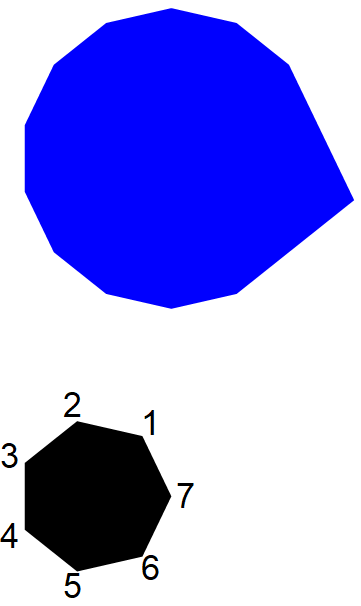
\includegraphics[width=0.6\linewidth]{meowmeow.png}}
\end{minipage}
\begin{minipage}[h]{0.49\linewidth}
\center{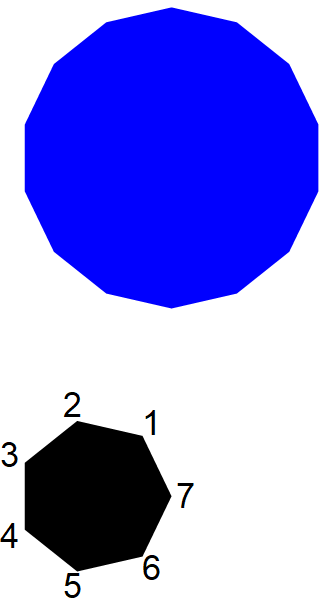
\includegraphics[width=0.5\linewidth]{meow.png}}
\end{minipage}
\caption{The left picture shows the polygon $S_{3625147}$, the right picture shows the polygon $S_{36251473625147}$, which is a periodic domain.}


\label{ris:image1}
\end{figure}

Point $(2, 3)$ is in the $S_{36251473625147}$ and it has a period ${36251473625147}$.

\begin{figure}[h!]
    \centering
    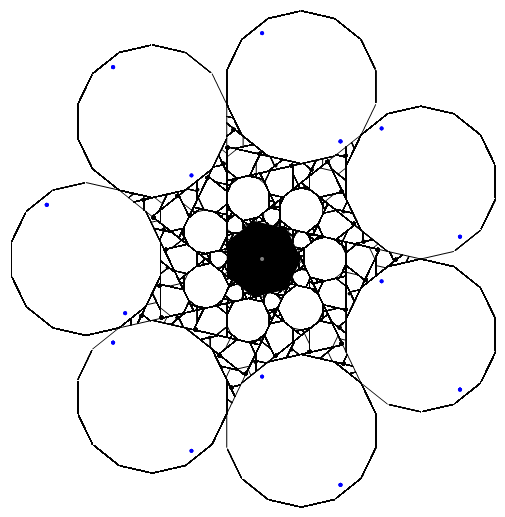
\includegraphics[width=0.6\linewidth]{(2,3).png}
    \caption{Blue points are the iterations of the point $(2, 3)$.}
    \label{fig:my_label}
\end{figure}


\newpage

\section{Characterization of the set of aperiodic points}
\begin{lemma}\label{apinbnd}
The set of aperiodic points is a subset of $Cl(B_{\infty})$.
\end{lemma}
\begin{proof}
Suppose that the statement of the lemma does not hold. Then there exists an aperiodic point $x$ and an open ball $B(x,r)$ centered at $x$ with radius $r>0$ such that $B(x,r)\cap B_{\infty} = \emptyset$. It is obvious by induction that for each $k \geq 0$ we have $f^k(B(x,r))=B(f^k(x),r)$, also, $f^k(B(x,r))$ does not intersect $B_{\infty}$ and, in particular, for each $k\geq 0$ the set $B(f^k(x),r)$ is a subset of some $D_{i(k)},\;1 \leq i(k) \leq 7$. Hence, all points in $B(x,r)$ have the same itinerary.

It is a well-known fact (follows from \cite{bounded}, Prop.1) that each point of an outer billiard with respect to a regular polygon has a bounded trajectory. Hence, for some $R>0$ all the balls $f^k(B(x,r))$ are subsets of $B(0,R)$, which means that there exist $0\leq k < l$ such that \[f^{2k}(B(x,r)) \cap f^{2l}(B(x,r))\neq \emptyset.\] As all points of $B(x,r)$ have the same itinerary, $f^k$ is injective on $B(x,r)$ for each $k \geq 0$. Hence, $f^{2(l-k)}(B(x,r)) \cap B(x,r) \neq \emptyset$. Moreover, for each $t \geq 0$, \[f^{2(l-k)t}(B(x,r))\cap f^{2(l-k)(t+1)}(B(x,r)) \neq \emptyset.\] Combining this with the fact that for each $t \geq 0$ all points in $f^{2(l-k)t}(B(x,r))$ have the same itinerary, we conclude that each two points $x,y \in \bigcup\limits_{t=0}^{\infty} f^{2(l-k)t}(B(x,r)) $ have the same itinerary. Hence, $f^{2(l-k)}$ acts on $\bigcup\limits_{t=0}^{\infty} f^{2(l-k)t}(B(x,r))$ as a parallel translation. So, if this parallel translation is not equal to the identity transform, then $f^{2(l-k)t}(x)=x+tv$ for all $t \geq 0$ and some vector $v$.
If $v \neq 0$, then the set $\bigcup\limits_{t=0}^{\infty} f^{2(l-k)t}(x)$ is unbounded, in particular, the orbit of $x$ is unbounded, and we get a contradiction with \cite{bounded}, Prop.1. Hence, $v=0$ and $f^{2(l-k)}(x)=x$, so $x$ is periodic, which is also a contradiction.
\end{proof}

On the other hand, as we have seen before, the set of periodic points is open, hence, it does not contain any points from $Cl(B_{\infty})$. Combining this with Lemma \ref{apinbnd}, we conclude that the set of aperiodic points coincides with $Cl(B_{\infty})\backslash B_{\infty}$.

In the future we are planning to get some additional information about the sets of periodic, aperiodic, and boundary points. In particular, two questions seem interesting: 

1) Is it true that $Cl(B_{\infty})$ is nowhere dense?

2) Is it true that $Cl(B_{\infty})$ has Lebesgue measure 0?

In the case of a regular pentagon, the answer to these questions is positive, the proof is based on multiple similarities in the dynamics of some fragments of the outer billiard, but in the case of a 7gon it seems much harder to find analogous similarities.

\begin{thebibliography}{}
\bibitem{bounded} F. Vivaldi, A. Schaidenko, \emph{Global stability of a class of discontinuous dual billiards}, Comm. Math. Phys. \textbf{110} (1987) 625-640
\end{thebibliography}


\end{document}
